%-----------------------------------------------------------------
%	INTRODUCTION
%	!TEX root = ./../main.tex
%-----------------------------------------------------------------
\section{Introduction}
\subsection{Lorentz classical model}
In this model (figure \ref{fig:lorentz-model}), the force that acts upon the electron is modelled as a recovery force:
\begin{align}
	\va{F} = - k \va{r} \, \overset{1D}{\longmapsto} \, F = - k x
\end{align}
\begin{figure}[H]
	\centering
	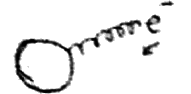
\includegraphics[width=0.2\textwidth]{./images/1-lorentz-model}
	\caption{Diagram of the Lorentz model for an atom}
	\label{fig:lorentz-model}
\end{figure}

Therefore, the equation of motion for the electron is
\begin{align*}
	\ddot{x} + \omega_{0}^{2}x = 0 \qc \omega_{0} = \sqrt{\frac{k}{m}} \Rightarrow x = A \cos(\omega_{0} t + \varphi)
\end{align*}
Introducing a damping term to account for the spontaneous emission, we get
\begin{align}
	\ddot{x} + \gamma \dot{x} + \omega_{0}^{2}x = 0
\end{align}

%-----------------------------------------------------------------
\subsection[Electric dipole approximation]{Electric dipole approximation (EDA)}
In the presence of an external electric field, $\va{E}(z,t) = E_{0} \cos(kz - \omega t) \vu{x}$, and introducing the oscillator strength, $f$, we can explain absorption and stimulated emission as well.

\begin{defi}[Oscillator strength]
	The oscillator strength, $f$, is a dimensionless quantity that expresses the probability of absorption or emission of electromagnetic radiation in transitions between energy levels of an atom or molecule.
	\begin{align*}
		f &> 0 \Rightarrow \text{ absorption} \\
		f &< 0 \Rightarrow \text{ stimulated emission}
	\end{align*}
\end{defi}

The force that acts upon a charged particle in the presence of an electric field is $\va{F} = q \va{E}$, therefore, we get
\begin{align*}
	\ddot{x} + \gamma \dot{x} + \omega_{0}^{2}x = f \frac{e E_{0}}{m} \cos(kz - \omega t)
\end{align*}

We can assume that the size of the atom is much smaller than the optical wavelength, so that the electron only sees the field at the nuclear position; this approximation is the so called electric dipole approximation. Therefore, $k z_{cm} \to 0$, and the previous equation becomes
\begin{align}
	\ddot{x} + \gamma \dot{x} + \omega_{0}^{2}x = f \frac{e E_{0}}{m} \cos(\omega t)
\end{align}

Consequently, we can get absorption or stimulated emission. Since $\dv*{W}{t} = - P$, we can study them measuring the mean value of the power in a cycle:
\begin{align}
	\ev{P} = \ev{F \dot{x}}
	\begin{cases}
		>0 & \text{(absorption)} \\
		<0 & \text{(stimulated emission)}
	\end{cases}
\end{align}
This models gives us $x(t)$.

\subsubsection*{Susceptibility}
In a homogeneous linear and isotropic dielectric medium, the polarization is aligned with and proportional to the electric field: $\va{P} = \varepsilon_{0} \chi \va{E}$. In a dipole, it can be written as $P = N e x$. Therefore, we can express the susceptibility as
\begin{align}
	\chi = \frac{N e x}{\varepsilon E} \equiv \chi' + i \chi''
\end{align}
The real part of the susceptibility, $\Re{\chi} = \chi'$ is related to index of refraction of the medium; the imaginary part, $\Im{\chi} = \chi''$ is related to the absorption coefficient.

\subsubsection*{Other media}
The natural frequency, $\omega_{0}$, gives us the model of the properties of the media. For metals, for instance, $\omega_{0} \to 0$ (electrons are not bound).

%-----------------------------------------------------------------
\subsection{Classical coherence}
\subsubsection*{First-order correlation function}
We can measure the coherence of an electric field with the help of an interferometer. In the figure \ref{fig:interferometer}, we see that $\va{E}_{1} = \va{E}(t)$, $\va{E}_{2} = \va{E}(t + \tau)$, and $\va{E}_{sum} = \va{E}_{1} + \va{E}_{2}$. So that, the intensity detected is $I \propto \ev{\va{E}^{2}_{sum}}$.
\begin{figure}[H]
	\centering
	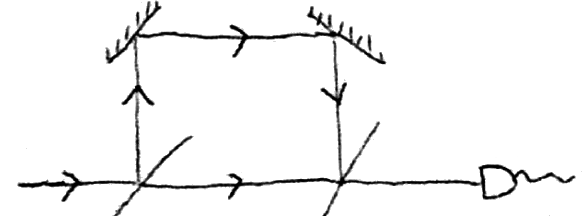
\includegraphics[width=0.5\textwidth]{./images/1-interferometer}
	\caption{Diagram of an interferometer with 50--50 beam splitters}
	\label{fig:interferometer}
\end{figure}

If we express $\va{E}(\va{r},t) = \va{E}^{(-}(\va{r},t) + \va{E}^{(-}(\va{r},t)$, where $\va{E}^{(+)} \equiv \va{E}^{(-)\sast}$, we can rewrite the expression for $I$:
\begin{flalign*}
	I & \propto \ev{(\va{E}_{1} + \va{E}_{2})^{2}} = \cdots = \ev{E^{(-)}_{1} E^{(+)}_{1}} + \ev{E^{(-)}_{2} E^{(+)}_{2}} + 2 \Re{ \ev{E^{(-)}_{1} E^{(+)}_{2}} } & \\
	& \Rightarrow I \propto 2 I_{0} + 2 \Re{E^{(-)}(t) + E^{(+)}(t + \tau)}
\end{flalign*}

\begin{defi}[First-order correlation function]
	\begin{align}
		G^{(1)}(t, t + \tau) \equiv \ev{E^{(-)}(t) + E^{(+)}(t + \tau)} = G^{(1)}(\tau)
	\end{align}
\end{defi}

The visibility is defined as $V = \dfrac{I_{max} - I_{min}}{I_{max} + I_{min}}$. Rewriting the first-order correlation function as $G^{(1)}(\tau) = \abs{G^{(1)}(\tau)} e^{i \phi(\tau)}$, we can easily work out $I_{max}$ and $I_{min}$:
\begin{flalign*}
	I & \propto 2 I_{0} + 2 \abs{G^{(1)}(\tau)} \cos[\phi(\tau)] \Rightarrow
	\begin{cases}
		I[\cos(\phi)] = -1 \Leftrightarrow I_{min} = 2I_{0} - 2 \abs{G^{(1)}(\tau)} \\
		I[\cos(\phi)] = +1 \Leftrightarrow I_{max} = 2I_{0} + 2 \abs{G^{(1)}(\tau)}
	\end{cases}
	 &
\end{flalign*}

\begin{defi}[Normalised first-order coherence function]
	We can rearrange the terms of the visibility to express it in terms of the first-order coherence function:
	\begin{align*}
		V = \dfrac{\abs{G^{(1)}(\tau)}}{\ev{E^{(-)}(t) E^{(+)}(t)}}
	\end{align*}
	this is what we call the normalised first-order coherence function, $g^{(1)}(\tau)$.
	\begin{align}
		V = \frac{I_{max} - I_{min}}{I_{max} + I_{min}} = \abs{g^{(1)}(\tau)}
		\begin{cases}
			= 0 & \Rightarrow \text{incoherent field} \\
			\in (0,1) & \Rightarrow \text{partially coherent field} \\
			= 1 & \Rightarrow \text{fully coherent field}
		\end{cases}
	\end{align}
\end{defi}

\subsubsection*{Second-order correlation function}
\begin{defi}[Normalised second-order correlation function]
	The degree of second-order correlation function is the autocorrelation function for the intensity, rather than the field. We can define this function as
	\begin{align}
		g^{(2)}(\tau) = \frac{\ev{ E^{(-)}(t) E^{(-)}(t + \tau) E^{(+)}(t + \tau) E^{(+)}(t) }}{\ev{ E^{(-)}(t) E^{(+)}(t) }}
	\end{align}
\end{defi}

%-----------------------------------------------------------------
\subsection{Hanbury--Brown--Twiss experiment}
One important feature of the second-order coherence function is that it can be measured with a reasonably simple set-up, the famous Hanbury--Brown–-Twiss apparatus (figure \ref{fig:hbt-experiment}). An input field is divided by a beam splitter, and the two components are monitored by two photo-detectors. The two detector signals are fed into a signal multiplier (mixer), though only after a variable time delay is added to one of the signals. The mixer signal is fed through a low-pass filter, which can be thought of as a integrator with a running time average.
\begin{figure}[H]
	\centering
	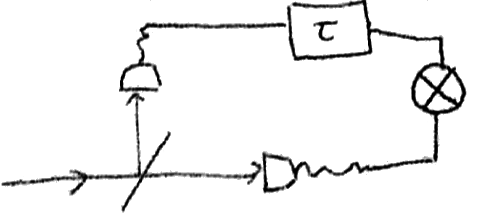
\includegraphics[width=0.4\textwidth]{./images/1-hbt-experiment}
	\caption{Diagram fo the Hanbury--Brown--Twiss experiment}
	\label{fig:hbt-experiment}
\end{figure}
This set-up, because it effectively correlates the two intensities, seems to give the $g^{(2)}(\tau)$ function as its output signal directly:
\begin{align}
	g^{(2)}(\tau) = \frac{\ev{I(t) I(t + \tau)}}{\ev{I(t)}^{2}}
\end{align}

\begin{align*}
	g^{(2)}(\tau)
	\begin{cases}
		\text{stationary field} & g^{(2)} (\tau) = 1 \\
		\text{fluctuating field} &
		\begin{cases}
			g^{(2)} (0) \geq 1 \\
			g^{(2)} (\tau) \leq g^{(2)} (0)
		\end{cases}
		\Rightarrow \text{bunching}
	\end{cases}
\end{align*}

\begin{figure}[H]
	\centering
	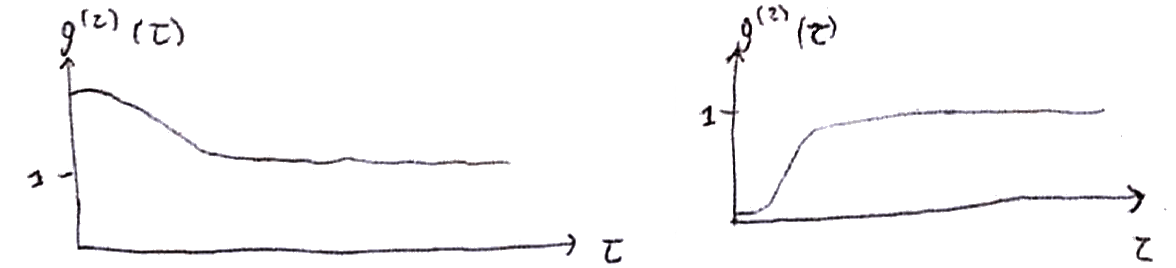
\includegraphics[width=\textwidth]{./images/1-bunching}
	\caption{(a) Bunching in a classical field, (b) antibunching in a quantum field}
	\label{fig:bunching}
\end{figure}
